\documentclass[border=1.5pt]{standalone}
\usepackage{amsmath,amssymb}
\usepackage{tikz}
\usetikzlibrary{arrows.meta,calc,positioning,shapes,shapes.misc,shapes.geometric,backgrounds,fit,decorations.pathreplacing,quantikz2}
% Shared colors and styles for the XYZ^2 figures.
% Pauli types: bright tones for fills and bands, deep (800) shades of the same hues for labels.
% The label shades keep the hue of each Pauli, are well separated from each other (CIEDE2000 > 20)
% and have a contrast ratio of at least 2.9 on the coral cells and 4.5 on the sunflower cells.
\definecolor{PauliX}{HTML}{F97316}
\definecolor{PauliY}{HTML}{EC4899}
\definecolor{PauliZ}{HTML}{9333EA}
\definecolor{PauliXText}{HTML}{AC340B}
\definecolor{PauliYText}{HTML}{9D174D}
\definecolor{PauliZText}{HTML}{5B21B6}
% Generator classes: S0 (class B, even links, coral) and gauge (class A, odd links, sunflower)
\definecolor{Szero}{HTML}{F0435E}
\definecolor{SzeroText}{HTML}{BE123C}
\definecolor{Gauge}{HTML}{F59E0B}
\definecolor{GaugeText}{HTML}{B45309}
\colorlet{GaugeGray}{Gauge}
\definecolor{ClassB}{HTML}{FF8A99}
\definecolor{ClassA}{HTML}{FFD23F}
% Logical operators (X-bar violet, Z-bar crimson), errors, ink
\definecolor{LogicalZ}{HTML}{E11D48}
\definecolor{LogicalGold}{HTML}{7C3AED}
\definecolor{ErrRed}{HTML}{1C1917}
\definecolor{InkDark}{HTML}{292524}
\definecolor{InkSoft}{HTML}{57534E}
% Labels drawn on top of colored cells
\colorlet{CellText}{InkDark}
% Noise channels
\definecolor{ErrFlip}{HTML}{EF4444}
\definecolor{Idle}{HTML}{EC4899}
\definecolor{TwoQ}{HTML}{7C3AED}
% Protocol steps
\definecolor{StepPrep}{HTML}{F97316}
\definecolor{StepMeas}{HTML}{D946EF}
\definecolor{StepDec}{HTML}{7C3AED}
\definecolor{StepRec}{HTML}{DB2777}
\tikzset{
  qb/.style={circle, draw=InkDark, line width=0.6pt, fill=white,
             minimum size=4.2mm, inner sep=0pt, font=\scriptsize},
  qbsmall/.style={circle, draw=InkDark, line width=0.5pt, fill=white,
             minimum size=2.6mm, inner sep=0pt},
  hexedge/.style={line width=0.65pt, draw=InkSoft},
  linkedge/.style={line width=1.6pt, draw=InkDark},
  bndedge/.style={line width=0.65pt, draw=InkSoft, densely dashed},
  plabel/.style={font=\scriptsize\bfseries, inner sep=1pt},
  panel/.style={font=\small\bfseries, anchor=north west},
}

\providecommand{\ket}[1]{\left|#1\right\rangle}

\begin{document}
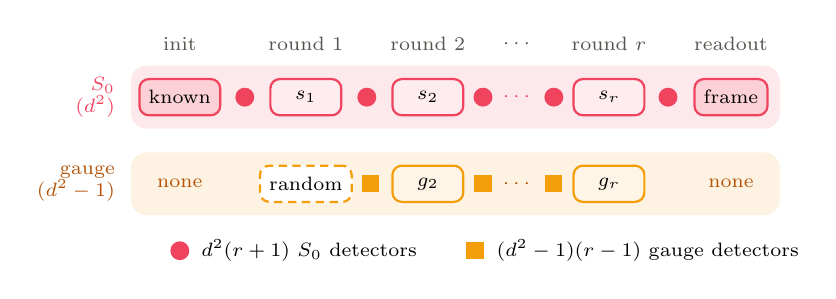
\begin{tikzpicture}[meas/.style={rounded corners=1.2mm, minimum width=0.9cm, minimum height=0.46cm, line width=0.8pt, font=\scriptsize},sdet/.style={circle, fill=Szero, minimum size=2.4mm, inner sep=0pt},gdet/.style={rectangle, fill=Gauge, minimum size=2.2mm, inner sep=0pt}]
\fill[Szero!12, rounded corners=2mm] (-0.62,-0.4) rectangle (7.62,0.4);
\fill[Gauge!12, rounded corners=2mm] (-0.62,-1.5) rectangle (7.62,-0.7000000000000001);
\node[font=\scriptsize, text=Szero, anchor=east, align=right] at (-0.7,0.0) {$S_0$\\ ($d^2$)};
\node[font=\scriptsize, text=GaugeText, anchor=east, align=right] at (-0.7,-1.1) {gauge\\ ($d^2-1$)};
\node[font=\scriptsize, text=InkSoft] at (0.0,0.68) {init};
\node[font=\scriptsize, text=InkSoft] at (1.6,0.68) {round 1};
\node[font=\scriptsize, text=InkSoft] at (3.15,0.68) {round 2};
\node[font=\scriptsize, text=InkSoft] at (4.3,0.68) {$\cdots$};
\node[font=\scriptsize, text=InkSoft] at (5.45,0.68) {round $r$};
\node[font=\scriptsize, text=InkSoft] at (7.0,0.68) {readout};
\node[meas, draw=Szero, fill=Szero!25] at (0.0,0.0) {known};
\node[font=\scriptsize, text=GaugeText] at (0.0,-1.1) {none};
\node[meas, draw=Szero, fill=Szero!10] at (1.6,0.0) {$s_1$};
\node[meas, draw=Gauge, fill=white, densely dashed] at (1.6,-1.1) {random};
\node[meas, draw=Szero, fill=Szero!10] at (3.15,0.0) {$s_2$};
\node[meas, draw=Gauge, fill=Gauge!10] at (3.15,-1.1) {$g_2$};
\node[font=\scriptsize, text=Szero] at (4.3,0.0) {$\cdots$};
\node[font=\scriptsize, text=GaugeText] at (4.3,-1.1) {$\cdots$};
\node[meas, draw=Szero, fill=Szero!10] at (5.45,0.0) {$s_r$};
\node[meas, draw=Gauge, fill=Gauge!10] at (5.45,-1.1) {$g_r$};
\node[meas, draw=Szero, fill=Szero!25] at (7.0,0.0) {frame};
\node[font=\scriptsize, text=GaugeText] at (7.0,-1.1) {none};
\node[sdet] at (0.825,0.0) {};
\node[sdet] at (2.375,0.0) {};
\node[sdet] at (3.850,0.0) {};
\node[sdet] at (4.750,0.0) {};
\node[sdet] at (6.200,0.0) {};
\node[gdet] at (2.425,-1.1) {};
\node[gdet] at (3.850,-1.1) {};
\node[gdet] at (4.750,-1.1) {};
\node[sdet] at (0.0,-1.95) {}; \node[font=\scriptsize, anchor=west] at (0.15,-1.95) {$d^2(r+1)$ $S_0$ detectors};
\node[gdet] at (3.75,-1.95) {}; \node[font=\scriptsize, anchor=west] at (3.9,-1.95) {$(d^2-1)(r-1)$ gauge detectors};
\end{tikzpicture}
\end{document}
